\documentclass[10pt]{article}
\title{Plant Generator}
\date{\today}
\usepackage[margin=1in]{geometry}
\usepackage{svg}
\usepackage{calc}
\usepackage{float}
\usepackage{amsmath}
\usepackage{pgfplots}
\pgfplotsset{compat=1.16}
\usepackage{fancyhdr}
\pagestyle{fancy}
\fancyhf{}
\fancyhead[L]{\leftmark}
\fancyhead[R]{\thepage}
\renewcommand{\footrulewidth}{0pt}
\renewcommand{\headrulewidth}{0.5pt}
\newcommand\m[1]{\begin{bmatrix}#1\end{bmatrix}}
\makeatletter
\begin{document}
\begin{center}
 \includesvg{resources/icon.svg} \\
 \vspace{1em}
 \begin{huge} \@title \end{huge} \\
 \vspace{1em}
 \@date
\end{center}
\tableofcontents
\pagebreak

\section{Introduction}
The project is split in two parts. The editor handles all user input and provides realtime feedback. It defines widgets, commands, selection types, and data structures for rendering. The plant generator generates plant structures and meshes, and it provides a means to export the result.
\begin{figure}[H]
\centering
\includesvg{resources/diagrams/outline.svg} \\
\caption{A high-level overview of the program.}
\end{figure}

\section{Background}
\subsection{Stems}
Auxin (IAA) lengthens cells by increasing cell wall elasticity. It is transported away from light through the shifting of PIN proteins in cell membranes. This process results in stems bending towards light. A common hypothesis is that auxin determines the apical dominance of the plant through a source-sink model. Fully saturating stems with auxin prevents axillary buds from releasing auxin into the stem and prevents further growth. The effects of auxin are countered with cytokinins (CK) that stimulate growth.

Formation of reaction wood is required for stems to grow upward or otherwise stems will bend down as their mass increases. Angiosperms produce tension wood in the upper part of the stem. Gymnosperms produce compression wood in the lower part of the stem. A stem under apical control develops only enough reaction wood to retain its angle but not enough to grow upward. Reaction wood enables one of the axillary stems to become the new central leader if the apical node is removed.

The apical meristem exhibits determinate growth if it produces a flower. The loss of apical control causes sympodial branching. Monopodial branching occurs when the apical meristem exhibits indeterminate growth. Dichotomous branching occurs when the apical node splits in two.

Growth is limited by the nitrogen concentration of the soil. More energy is put into roots when nitrogen is scarce and more stems are grown when nitrogen is abundant. There are other factors that affect growth such as altitude and temperature. Plants with needle-like leaves will resist freezing and water loss but not absorb as much sunlight.

\subsubsection{Terms}
\begin{itemize}
\item \texttt{Phytomer}: a unit containing a node, internode, and axillary bud
\item \texttt{Orthotropic}: vertical growth
\item \texttt{Plagiotropic}: horizontal growth
\item \texttt{Anisotropic}: unequal growth in different directions
\item \texttt{Isotropic}: equal growth in all directions
\item \texttt{Excurrent}: the plant maintains a single central leader
\item \texttt{Decurrent}: lateral stems compete with the central leader
\item \texttt{Acrotony}: stems first develop near the apex
\item \texttt{Mesotony}: stems first develop in the center
\item \texttt{Basitony}: stems first develop at the base
\item \texttt{Inflorescence}: a cluster of flowers including the stem
\item \texttt{Tortuous}: containing twists and turns
\item \texttt{Furrowed}: describes some bark textures
\end{itemize}

\subsection{Leaves}
The shape of a leaf is partly influenced by venation. The veins are composed of xylem cells (for the transportation of water) and phloem cells (for the outward transportation of sugars). Major veins provide support for the leaf and extend from the petiole to the leaf apices. Parallel venation can sometimes be seen in secondary veins, while minor veins form a network or a reticulate pattern. Minor veins can connect secondary veins creating loops.

The edge of a leaf is termed the leaf margin. Margins, for example, can be smooth, serrated, or sinuous. The margins and the overal shape are commonly used to determine what species a plant is. Alder, Elm and Birch trees have serrated leaves, and several oak species have sinuate leaves. Some leaf shapes are elliptic, deltoid, cordate, orbicular, or lobed. If a leaf is lobed, the tips can be either pointed or rounded.

\subsubsection{Terms}
\begin{itemize}
\item \texttt{Lamina}: the leaf surface
\item \texttt{Pinnate}: a feather-like arrangement
\item \texttt{Palmate}: a hand-shaped arrangement
\item \texttt{Craspedodromous}: secondary veins that extend towards the leaf margins
\item \texttt{Parallelodromous}: secondary veins that converge at the leaf apex
\item \texttt{Phyllotaxis}: the arrangement of leaves
\item \texttt{Acropetal}: leaves and flowers start developing at the top
\item \texttt{Basipetal}: leaves and flowers start developing at the bottom
\end{itemize}

\section{Generator}
\subsection{Iterative Growth Model}
A plant is grown over a certain number of growth cycles. A bounding box is generated at the beginning of each cycle and is used to construct a dome (the sky). Rays (light) originating on the dome intersect leaves to determine the efficiency of each stem in the plant. A stem is efficient if many intersections occur with its leaves and is grown by a random growth factor. Otherwise, if a stem receives no or little ray intersections, then the stem is shedded by the plant (known as cladoptosis). Remaining stems will grow in the average directions of rays that intersect with their leaves.

Each stem develops buds at the beginning of each iteration. Leaves form along the dormant nodes in the current iteration, and stems grow from the nodes in the following iteration. As stems grow older, a branch collar (swelling) forms at the base to secure the stem to the parent stem. Additionally, growth of lateral stems is suppressed by some factor depending on the distance to the apex of the parent stem. This suppression factor is intended to approximate the effects of auxin hormones that control the apical dominance of the plant.

\subsubsection{Irradiance}
The space the plant grows is partitioned using an octree. By recording how to the space is utilized, by the plant itself and surrounding objects, stems can be distributed more evenly throughout the space. Additionally, ray tracing volumes in the octree provides more information to the plant so that it can direct stems towards well illuminated volumes.

\begin{figure}[H]
 \begin{minipage}[t]{0.48\textwidth}
  \centering
  \includesvg{resources/diagrams/octree_node.svg}
  \caption{The next node in the octree is determined by comparing the ray direction against the face normals of the volume. A corner in the volume is selected based on the signs of the dot products of the ray direction and normals.}
 \end{minipage}
 \hfill
 \begin{minipage}[t]{0.48\textwidth}
  \centering
  \includesvg{resources/diagrams/octree.svg} \\
  \caption{The plant is first stored in an octree and then the radiant flux through each volume is calculated by casting rays through the space.}
 \end{minipage}
\end{figure}

\begin{figure}[H]
\begin{minipage}[t]{0.48\textwidth}
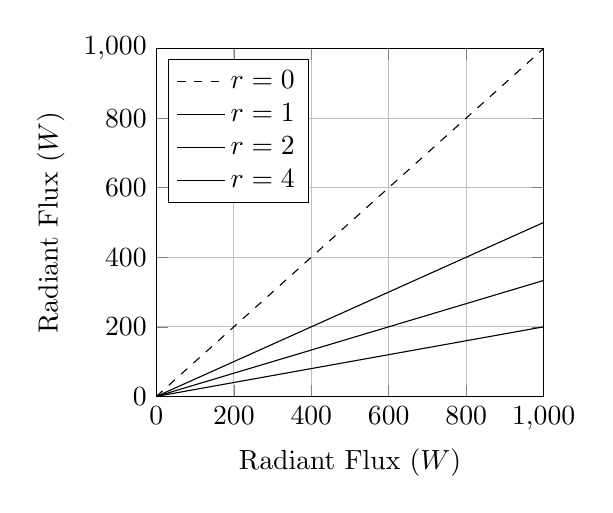
\begin{tikzpicture}
\begin{axis}[height=6cm, width=6.5cm, xmin=0, xmax=1000, ymin=0, ymax=1000, xtick={0, 200, 400, 600, 800, 1000}, ytick={0, 200, 400, 600, 800, 1000}, grid=both, legend pos=north west, xlabel={Radiant Flux ($ W $)}, ylabel={Radiant Flux ($ W $)}]
\addplot [domain=0:1000, samples=2, style=dashed]{x/(1)};
\addlegendentry{$ r = 0 $}
\addplot [domain=0:1000, samples=2]{x/(1+1)};
\addlegendentry{$ r = 1 $}
\addplot [domain=0:1000, samples=2]{x/(1+2)};
\addlegendentry{$ r = 2 $}
\addplot [domain=0:1000, samples=2]{x/(1+4)};
\addlegendentry{$ r = 4 $}
\end{axis}
\end{tikzpicture}
\caption{The densisty ($ r $) of each volume in the octree reduces the radiant flux within the canopy.}
\end{minipage}
\hfill
\begin{minipage}[t]{0.48\textwidth}
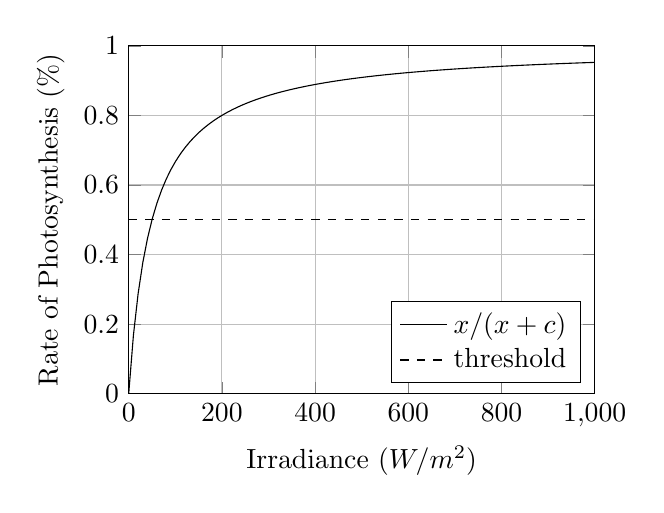
\begin{tikzpicture}
\begin{axis}[height=6cm, width=7.5cm, xmin=0, xmax=1000, ymin=0, ymax=1, grid=both, legend pos=south east, xlabel={Irradiance ($ W/m^2 $)}, ylabel={Rate of Photosynthesis (\%)}]
\addplot [domain=0:1000, samples=100]{x/(x+50)};
\addlegendentry{$x/(x+c)$}
\addplot [domain=0:1000, samples=2, style=dashed]{0.5};
\addlegendentry{threshold}
\end{axis}
\end{tikzpicture}
\caption{The photosynthesis-irradiance curve shows how irradiance influences the rate of photosynthesis. A threshold denotes the minimum efficiency.}
\end{minipage}
\end{figure}

\subsubsection{Hormones}
The rate of stem growth is determined by hormone concentrations. Some hormones, such as auxins, are produced in the apical nodes of stems. Other hormones, such as strigolactones and some cytokinins, are produced in the roots of the plant. Therefore, rates of growth are determined by both bottom-up and top-down processes.

Assume that each apical node produces a fixed amount of hormones. Also assume that each stem can only transport chemicals up to some threshold and that this threshold is proportional to the radius of the stem. Let $ R $ be the radius function, $ l $ be the length of a stem, and $ h $ be the quantity of some hormone.

\[ R(x) = 1 - \frac{x}{l} \]
\[ V(x) = \int \pi R(x)^2 dx = \frac{-\pi l}{3} \left( 1 - \frac{x}{l} \right)^3 + c \]
\[ 0 \leq \frac{h(b-a)}{V(b)-V(a)} \leq 1 \]

\subsection{Stems}
The positions of stems are stored as distances along parent stems. Stems internally calculate their location in the world space when distances are changed and when the paths of ancestor stems are changed. Some resources, such as materials and curves, are referenced with indices. The indices point to resources located in the plant object.

\subsubsection{Materials}
The plant object stores a list of all materials that stems and leaves can have. Stems and leaves store indices of materials so that they only have to be updated in the plant object. The geometry generator needs to create vertex seams (i.e., duplicate vertices) so that textures can be wraped around the stems.

\subsubsection{Bark Ridges and Branch Collars}
The branch collar is a swelling at the base of the stem that increases the structural integrity of the joint. The bark ridge can be generated by using two B\'{e}zier curves, but that would require finding a third point and increasing the complexity of the algorithm.

\setlength{\parindent}{1.5em}
A cone intersection test (for tapered cylinders) can be used to fuse one stem to the other, but this is only ideal if the cross sections are guaranteed to be circular. Triangle intersection tests will work for all shapes but with the cost of worse performance. To increase performance, intersections should start at the the location of the stem and move outwards towards the top and bottom of the parent stem. If triangle intersections only pass when a ray intersects with the front sides of triangles, then the first intersection is likely to be the correct one.

\begin{figure}[H]
 \begin{minipage}[H]{0.46\textwidth}
The normals along the collar are interpolated using a piecewise function that resembles a sigmoid function, but such that $ f: \left[ 0, 1 \right] \rightarrow \left[ 0, 1 \right] $.
\[ f(x) =
\begin{cases}
(\sqrt{2}x)^2 & 0 \leq x \leq \frac{1}{2}\\
-\left[\sqrt{2}(x-1)\right]^2 + 1 & \frac{1}{2} \leq x \leq 1 \\
\end{cases} \]
 \end{minipage}
 \hfill
 \begin{minipage}[H]{0.46\textwidth}
  \centering
  \includesvg{resources/diagrams/collar.svg} \\
  \caption{The first cross section is scaled along the parent stem direction (1) and is intersected with the parent's surface (2). A spline connects the transformed cross section with the second cross section (3).}
 \end{minipage}
\end{figure}

\subsubsection{Bifurcation}
\begin{enumerate}
\item The first stem is to avoid overlapping cross sections. Assuming that the paths are lines, the law of sines can be used to find a distance wherein no cross sections should be generated. Let $ d $ be the distance, $ r $ be the radius, and $ \theta $ be the angle between the vectors (Figure \ref{fig:forkside}).
\[ d = r \cdot \frac{\sin[(\pi-\theta)\div2]}{\sin (\theta\div2)} \]
A more flexible approach is to project points along one path onto the other path and measure the distances. The paths are evaluated in an alternating manner so that the algorithm exits the first time the paths stop intersecting so that not all points need to be evaluated. Alternation occurs whenever a check fails (Figure \ref{fig:path}).

Another approach is to assume that the cross section are not overlapping. Cross sections between the first two control points of the stem path are eliminated, and the second control point is calculated in a manner that avoids overlapping.

\begin{figure}[h]
 \begin{minipage}[b]{0.46\textwidth}
  \centering
  \includesvg{resources/diagrams/fork_side.svg}
  \caption{The length of the top edge of the shaded triangle is the distance that is required to be free of cross sections.} \label{fig:forkside}
 \end{minipage}
 \hfill
 \begin{minipage}[b]{0.46\textwidth}
  \centering
  \includesvg{resources/diagrams/path.svg}
  \caption{Points along one path are projected on the line segments of the second path. The paths intersect when the distances of the projections are less than the diameter of the cross sections and the projected points fall within the line segments.} \label{fig:path}
 \end{minipage}
\end{figure}

\item The second step is to find two points on the cross section that will divide it in half. To avoid the situation illustrated in Figure \ref{fig:fork2}, it is necessary for cross sections to be rotated relatively to each other (i.e., subsequent rotations are concatenated with previous rotations).

The cross section is rotated into the average of the two stem direction vectors (Figure \ref{fig:forkdiv}). One of the two child vectors is then projected on the plane of the cross section. Then, the angle between the projected vector and the first point on the cross section is measured. The range of the inverse cosine function is $ [0, \pi] $, so it takes two dot products to determine an angle $ \theta $ in $ [0, 2\pi] $.

This method stops working reliably when a vector points in the opposite direction of the parent stem direction (boundary points can get flipped). To select a better frame of reference, three dot products are taken with the average of all three (outward pointing) vectors. The smallest dot product becomes the parent cross section.

\[ \text{midpoint} = \left\lfloor \frac{\theta}{2\pi \div \text{number of points}} \right\rceil \]

\begin{figure}[H]
 \begin{minipage}[b]{0.49\textwidth}
  \centering
  \includesvg{resources/diagrams/fork_section.svg}
  \caption{Rotating the cross section into the average direction of the two forks is necessary to determine where the cross section needs to be divided in half.} \label{fig:forkdiv}
 \end{minipage}
 \hfill
 \begin{minipage}[b]{0.48\textwidth}
  \centering
  \includesvg{resources/diagrams/fork_resolution.svg}
  \caption{Rounding to the nearest integer is required when $ n \bmod 4 = 0 $ and otherwise \texttt{floor} or \texttt{ceil} is required.}
 \end{minipage}
\end{figure}
\begin{figure}[H]
 \begin{minipage}[H]{0.24\textwidth}
  \centering
  \includesvg{resources/diagrams/fork1_topdown.svg}
  \caption{Points are connected without distortion.} \label{fig:fork1}
 \end{minipage}
 \hfill
 \begin{minipage}[H]{0.24\textwidth}
  \centering
  \includesvg{resources/diagrams/fork2_topdown.svg}
  \caption{Points cannot be connected without distortion.} \label{fig:fork2}
 \end{minipage}
 \hfill
 \begin{minipage}[H]{0.4\textwidth}
  \centering
  \includesvg{resources/diagrams/fork3_topdown.svg}
  \caption{Points are connected without distortion but two extra triangles are needed.} \label{fig:fork3}
 \end{minipage}
\end{figure}

\item Cross sections are projected onto three planes so that pairs of points overlap. Cross sections can also be connected with B\'{e}zier curves if the projected points are used as tangent points.
\end{enumerate}

\subsection{Leaves}
The positions of leaves are stored as distances along the parent stem. The world positions of leaves can only be determined if the parent stems are also known because leaves do not know about their parent stems. Additionally, each leaf is defined by a mesh which contains a set of points, indices, and texture coordinates. These meshes are stored within the plant object and are inserted into the plant geometry during mesh generation.

\subsubsection{Rotations}
\begin{minipage}[t]{0.6\textwidth}
Cross products can be used to derive the rotations of leaves, but only in the absence of parallel vectors. For example, the cross product of the up vector and the stem direction is undefined if both vectors are identical. A more performance intensive solution is to derive the final rotation by concatenating multiple quaternion rotations. Some considerations to determine to rotations of leaves are:
\begin{itemize}
\item Leaves tend to point in the same direction as shoots because shoots grow towards light.
\item The locations of buds influence the rotations of leaves, although petioles reduce this influence.
\end{itemize}
\end{minipage}
\hfill
\begin{minipage}[t]{0.3\textwidth}
 \begin{figure}[H]
  \centering
  \includesvg{resources/diagrams/leaves.svg}
  \caption{Leaf rotations are influenced by the locations of leaf buds. This diagram ignores the function of petioles.}
 \end{figure}
\end{minipage}

\section{Editor}
\subsection{Camera}
The camera produces matrices for transforming the world space into the screen space. It also produces inverse matrices so that the screen space can be transformed back into the world space. This is useful for object selection.
\begin{itemize}
\item \texttt{Vec3 target}: The point the camera is pointed at.
\item \texttt{float distance}: The distance the camera is from the target.
\item \texttt{float x}: A rotation around the x-axis.
\item \texttt{float y}: A rotation around the y-axis.
\end{itemize}
The \texttt{x} and \texttt{y} rotations are used to calculate a point on a sphere. The location of the camera is therefore: (\textit{location on sphere}) (\textit{distance}) + \textit{target}. The \texttt{x} and \texttt{y} rotations are also used to maintain the orientation of the camera even when the view direction and up vectors are parallel.

\subsection{Commands}
The editor uses the command pattern to store all user invocable commands. This allows each command to be easily associated with a key combination, and this makes it possible to implement an undo/redo system without having to copy the entire application state. Commands are required to have execute, undo, and redo methods. The downside of this approach is that the the undo behavior of prior commands will be wrong if a command improperly undoes its changes.

\subsubsection{Move Commands}
The cursor position is converted into a ray pointing into the world space in order to move an object in the world space using the cursor. The ray is used to create a point in the world space by intersecting with a plane that is parallel to the camera direction. Points are moved by the difference of the initial and last (cursor generated) points.

There is also a need to move points along paths instead of straight through the world space. This functions differently from the first method. Instead of converting the cursor position to a point in the world space, the points along the path are converted to the screen space. The cursor position is projected onto the (now two-dimensional) path to determine a new point.

\subsubsection{Save Commands}
The internal properties of stems and leaves can be adjusted using a property editor. The program checks for changes within the selection whenever a property editor loses focus. A save command storing the original objects is inserted into the history if changes were made.

\subsubsection{Generator Commands}
Ideally, a generator command should not have to store generated objects in order to be able to redo the program state. The following options would increase the program complexity in one way or another.

\begin{itemize}
\item If objects are identified by IDs, then the generator would have to be able to create objects with the same IDs. Some operations, such as reinserting stems, would require a lookup operation.
\item If objects are identified by memory address, then an object pool is required for objects to be freed and reallocated at the same address. The order of the pool's free list will change if objects are not removed in the opposite order of the allocation order. This will cause commands in the redo stack to operate on invalid selections. Other commands also have to revert the free list to the previous order in order to maintain valid selections.
\end{itemize}

\subsection{Selection}
The selection object contains structures for storing stem, point and leaf selections. The user creates a selection through a selector object. Removing camera and other scene information from the selection decreases the size of the history and coupling. Commands can update the selection directly through the selection object.

\subsection{Resources}
A \texttt{SharedResources} object stores all the shader programs and materials that are needed across all OpenGL widgets. Default images are automatically loaded from the \texttt{resources} file, and shaders are automatically loaded from the \texttt{shaders} file. Signals are emitted whenever materials are modified so that property editors can adjust their combo boxes to match the global state.

\subsection{History}
The history maintains a list of past and future commands. The timestamps within commands are used to verify that new commands are more recent than the previous command. Commands can be flipped if their timestamps are out of order, which could happen if they are added to the history during focus events.

\section{Shaders}
\subsection{Outlines}
Selected objects are indicated with an outline around their silhouette. The outline is achieved in two passes. The first pass draws the selected objects offscreen in solid white onto a black background. This image is stored in a texture for the second pass. During the second pass, the fragment shader refers to this texture to determine if a fragment is close to the object's silhouette edge. Even though the fragment shader needs to scan and analyze the texture, it needs to avoid branch divergence in order to keep performance acceptable.

\end{document}
